\documentclass[12pt]{article}

\usepackage[utf8]{inputenc}
\usepackage[english, russian]{babel}
\usepackage{minted}

% "А вот теперь --- слайды!"
\usepackage{slides}

\usepackage{graphicx}
\usepackage{pdfpages}

\def\Person{Шапошников А.А.}
\def\Title{Тесты во фронтике}
\def\FooterTitle{\Title}
\def\SubTitle{Пара идей о том, как можно тестировать приложения frontik}
\newcommand{\TitleSlide}{
    \addcontentsline{toc}{section}{\Title}%
    ~\vspace{1cm}

    \begin{center}
    {\huge \begin{spacing}{1}\Title\end{spacing}}

    {\SubTitle}
    \vspace{2cm}

    \ifthenelse{\isundefined{\Student}}{}
        {\small Студент: \Student\\}
    \ifthenelse{\isundefined{\Advisor}}{}
        {\small Руководитель: \Advisor\\}
    \ifthenelse{\isundefined{\Person}}{}
        {\Person\\}
    \ifthenelse{\isundefined{\Affilation}}{}
        {\Affilation\\}
    \end{center}
    \thispagestyle{empty}
}


%% Переносы в презентации смотряся не очень.
\hyphenpenalty 10000
\sloppy


% pygments какие-то стили
% /pygments

\usepackage{fontspec} % loaded by polyglossia, but included here for transparency
\usepackage{polyglossia}
\setmainlanguage{russian}
\setotherlanguage{english}

% XeLaTeX can use any font installed in your system fonts folder
% Linux Libertine in the next line can be replaced with any
% OpenType or TrueType font that supports the Cyrillic script.
\setromanfont[Mapping=tex-text]{Liberation Serif}
\setsansfont[Mapping=tex-text]{Liberation Sans} % Without this Cyrillic Sans Serif text won't show.
\setmonofont[Mapping=tex-text]{Nimbus Mono L}


\begin{document}


\includegraphics{logo.png}
\TitleSlide

\section{Мотивация и цель}
"TDD во фронтике"

Обеспечить слой logic системой, позволяющей отлавливать баги связанные с изменением контрактов с внешними сервисами

В целом дружить с нашей экосистемой

\section{Требования к тестам}

\begin{enumerate}
\item Наглядность и читаемость, совместимость с unittest инфраструктурой python
\item Не должны зависеть от способа их запуска и чего-то требовать от окружения (т.е. unit тесты)
\end{enumerate}

\section{}
\begin{figure}[ht!]
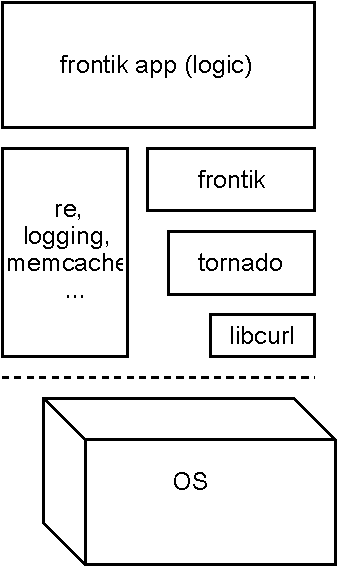
\includegraphics[page=1, scale=1.6]{frontikarchitecture.pdf}
%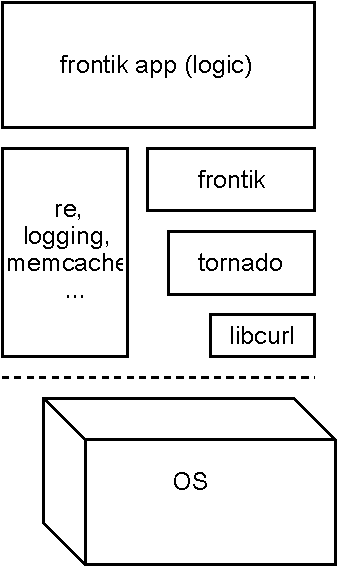
\includepdf[page=1]{frontikarchitecture.pdf}
\end{figure}

\section{Тестовый фреймворк}

\begin{itemize}
\item Приложения frontik ходят в бэкэнды, затем опционально накладывают xsl
\item Такая узкая специализация позволяет встроиться и перехватывать запросы в сетевом стеке и приложение изолировано

\end{itemize}

\section{}
\begin{figure}[ht!]
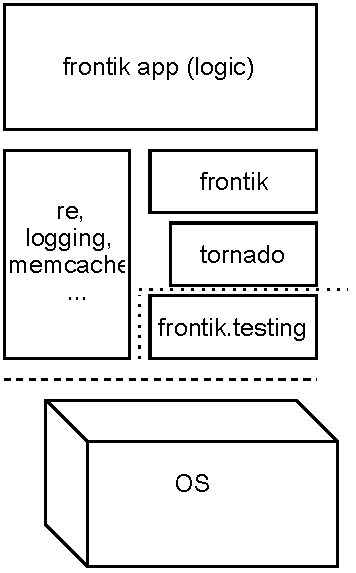
\includegraphics[page=1, scale=1.6]{frontiktesting.pdf}
%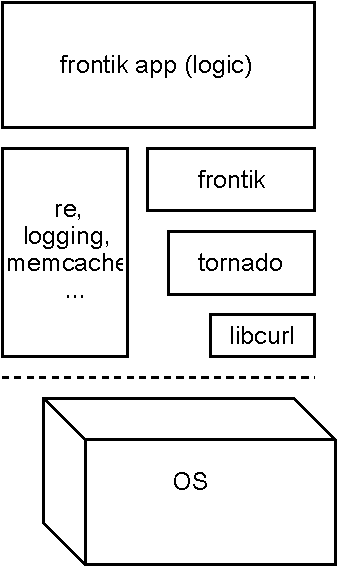
\includepdf[page=1]{frontikarchitecture.pdf}
\end{figure}

\section{}
\begin{figure}
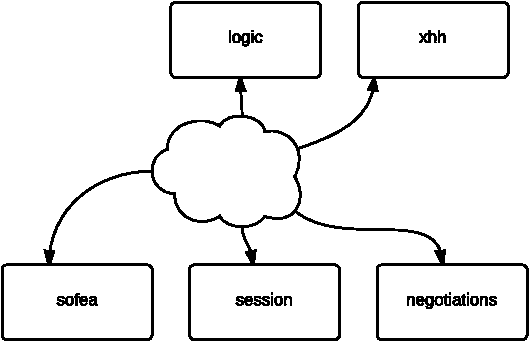
\includegraphics[page=1, scale=2]{interconnection.pdf}
%\includepdf[pages={1}]{}
\end{figure}

\section{Ключевые решения в ходе разработки}

\begin{itemize}
\item Встроен во frontik. Использует настоящий экземпляр frontik c подмененным http-client
\item \emph{Нет} tornado/ioloop, callback'и вызываются через тестовый фреймворк
\item \emph{Нет} HTTP и сокетов, http-client напрямую ходит к мокам сервисов
\item собственно наложение xsl можно тестировать, но зачем?

\end{itemize}

\section{Стандартный подход к тестированию}
\begin{itemize}
\item setUp подготавливает общую часть

\item caveat: не поддерживается более одного вызова call в одном тесте
\end{itemize}

\section{Код под тестом}
\small
\inputminted[linenos=true]{python}{code.py}

\section{Тесты}

\small
\inputminted[linenos=true]{python}{test.py}

\verb+vacancies_by_manager+ - это метод под тестом

\verb+env+, \verb+EmptyEnvironment+ - импортированы из frontik.testing
\verb+call+ - позволяет вызвать тестируюемую функцию в подготовленном окружении

\section{Вызов тестирования интеграционного слоя}

Почти все тесты ходят за одними и теми же данными (i.e. вакансия, сессия), и в то же время не всем подойдет один и тот же ответ

Ответы генерируют внешние сервисы, которые лежат в другом репозитории и обновляются в случайный момент времени

Если контракт одного HTTP ресурса поменялся с одной стороны, тесты (в идеальном мире) показывают, что код, существенно его использующий на другой стороне, сломался

Как ориентироваться в моках?

\section{Репозиторий моков}

Напротив, развязан c frontik'ом и даже по возможности с питоном

Как оказалось, одного xml мало, мы храним рядом с ним ещё и необходимые header'ы

И ещё отдельно пару сервис-ресурс (aka host-url)

\section{Куда можно двигаться дальше}

\begin{enumerate}
\Large \item Документация
\item \normalsize  Более внятные сообщения об ошибках
\item \small Поддержка более широкого интерфейса, например IO loop
\item \small Версионность моков
\item \footnotesize "Встроенная" поддержка protobuf
\item \tiny Автоматизированный прогон тестов всех репозиториев после изменений в моках
\item \scriptsize Больше сахара, чтобы тесты не выглядели так страшно
\item \scriptsize Автоматическое определение race conditions
\item \scriptsize ...




\end{enumerate}

\section{Предлагаю критиковать}
Что пошло не так

\end{document}

